% Created 2018-06-21 Thu 12:30
\documentclass[8pt]{beamer}
\usepackage{pgfpages}

% ENABLE THIS FOR NOTES
\setbeameroption{show notes on second screen=right} % Both

\usepackage[sc,osf]{mathpazo}   % With old-style figures and real smallcaps.
\linespread{1.025}              % Palatino leads a little more leading
% Euler for math and numbers
\usepackage[euler-digits,small]{eulervm}
%\documentclass[10pt]{llncs}
%\usepackage{llncsdoc}
\usepackage{hyperref}
\usepackage{minted}
%\usemintedstyle{xcode}
\usepackage[utf8]{inputenc}
\usepackage[T1]{fontenc}
\usepackage{fixltx2e}
\usepackage{graphicx}
\usepackage{longtable}
\usepackage{float}
\usepackage{wrapfig}
\usepackage{rotating}
\usepackage[normalem]{ulem}
\usepackage{amsmath}
\usepackage{textcomp}
\usepackage{marvosym}
\usepackage{wasysym}
\usepackage{amssymb}
\usepackage{polynom}
\usepackage{changepage}
\usepackage{lipsum}


\hypersetup{colorlinks=true,
    linkcolor = blue,
    urlcolor  = blue,
    citecolor = blue,
    anchorcolor = blue
}
\renewcommand{\mod}[1]{\left( \texttt{mod}~#1 \right)}
\newcommand{\cpp}[1]{\mintinline{cpp}{#1}}
\newcommand{\py}[1]{\mintinline{py}{#1}}
\newcommand{\raw}[1]{\mintinline{text}{#1}}
\newcommand{\hs}[1]{\mintinline{hs}{#1}}
\newcommand{\smallpt}{\texttt{smallpt}}
\newcommand{\Ray}{\texttt{Ray}}
\newcommand{\Refl}{\texttt{Refl}}
\newcommand{\main}{\texttt{main}}
\newcommand{\intersect}{\texttt{intersect}}
\newcommand{\intersects}{\texttt{intersects}}
\tolerance=1000
% \usetheme{Antibes}
\author{Davean Scies, Siddharth Bhat}
\date{November 4th, 2020}
\institute{Haskell Exchange}
\title{Optimizing \smallpt}
\hypersetup{
  pdfkeywords={},
  pdfsubject={},
  pdfcreator={Emacs 24.5.1 (Org mode 8.2.10)}}

  \usepackage{xcolor}

\usepackage{listings}

\newcommand{\lstbg}[3][0pt]{{\fboxsep#1\colorbox{#2}{\strut #3}}}
\lstdefinelanguage{diff}{
  basicstyle=\ttfamily\small,
  morecomment=[f][\lstbg{red!20}]-,
  morecomment=[f][\lstbg{green!20}]+,
  morecomment=[f][\textit]{@@},
  %morecomment=[f][\textit]{---},
  %morecomment=[f][\textit]{+++},
}


\begin{document}

\maketitle

\begin{frame}[fragile]{What is smallpt anyway?}
\pause
\begin{columns}
\begin{column}{0.48\textwidth}
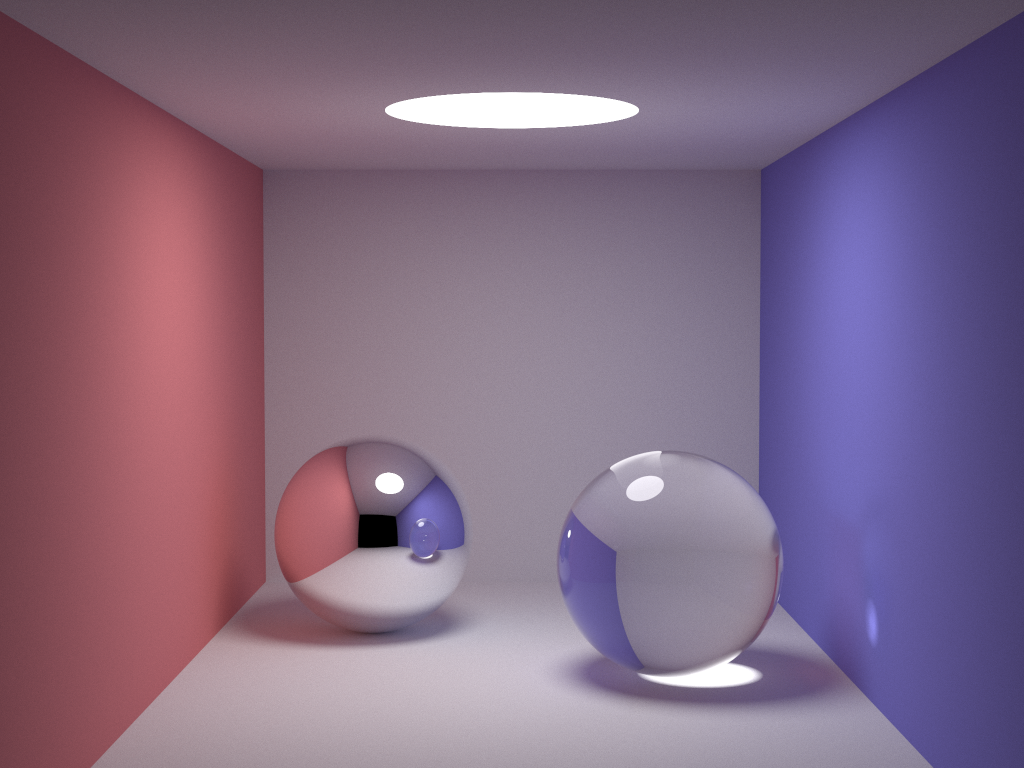
\includegraphics[height=0.8\textwidth]{./smallpt-render.png}
\end{column}
\begin{column}{0.48\textwidth}
\pause
\begin{itemize}
\item 100 LoC C demo of a raytracer \pause
\item Perfect for an optimization case study
\end{itemize}
\end{column}
\end{columns}
\end{frame}

\note{Note for first slide: what is smallpt anyway?}

\begin{frame}[fragile]{What is smallpt anyway?}
% \begin{adjustwidth}{-5em}{-5em}
\begin{minted}{cpp}
struct Vec {      
  double x, y, z; // position, also color (r,g,b) 
  ... methods...
}; 
struct Ray { Vec o, d; Ray(Vec o_, Vec d_) : o(o_), d(d_) {} }; 
enum Refl_t { DIFF, SPEC, REFR };  // material types, used in radiance() 
struct Sphere { 
  double rad;   // radius 
  Vec p, e, c;  // position, emission, color 
  Refl_t refl;  // reflection type (DIFFuse, SPECular, REFRactive) 
  ... methods ...
  double intersect(const Ray &r) const // returns distance, 0 if nohit 
}; 
Sphere spheres[] = {//Scene: radius, position, emission, color, material 
  Sphere(1e5, Vec( 1e5+1,40.8,81.6), Vec(),Vec(.75,.25,.25),DIFF),//Left 
  ... initialization ...
}; 
\end{minted}
% \end{adjustwidth}
\end{frame}


\begin{frame}[fragile]{What is smallpt anyway?}
\footnotesize
\begin{minted}{cpp}
Vec radiance(const Ray &r, int depth, unsigned short *Xi){ 
                                                                         
                                                                         
                                                                      
                                                               
                                                                           
                                                                            
                                                                            
                                                                         
                                                                   
                                                                     
                                                                      
                                                           
                                                                          
                                                                            
                                                                            
                                                                           
                                                                        
                                                                          
                                                          
                                                                          
                                                                           
                                                                            
                                                                            
                                                                          
                                                                         
} 
\end{minted}
\end{frame}

\note{Say that the core function is radiance}

\begin{frame}[fragile]{What is smallpt anyway?}
\footnotesize
\begin{minted}{cpp}
Vec radiance(const Ray &r, int depth, unsigned short *Xi){ 
                                                                      
                                                                      
                                                                   
                                                            
                                                                        
                                                                         
                                       
                                          
                                                                
                                                                  
                                                                   
                          radiance
                                          
                          radiance
                                                                         
                                                                        
                                                                     
                                         
                          radiance
                                                                       
                                                                        
                                                                         
                                                                         
    radiance                      radiance
    radiance                      radiance
} 
\end{minted}
\end{frame}

\begin{frame}[fragile]{What is smallpt anyway?}

\note{Say that it's recursive}
\footnotesize
\begin{minted}{cpp}
Vec radiance(const Ray &r, int depth, unsigned short *Xi){ 
                                                                      
                                                                      
                                                                   
                                                            
                                                                        
                                                                         
  if (         ) if (             )            else 
  if (                ){                  
                                                                
                                                                  
                                                                   
                          radiance
  } else if (                )            
                          radiance
                                                                         
                                                                        
                                                                     
  if (                               )   
                          radiance
                                                                       
                                                                        
                                                                         
                                                                         
    radiance                      radiance
    radiance                      radiance
} 
\end{minted}
\end{frame}

\note{...with control flow}

\begin{frame}[fragile]{What is smallpt anyway?}
\footnotesize
\begin{minted}{cpp}
Vec radiance(const Ray &r, int depth, unsigned short *Xi){ 
                                                                      
                                                                      
                                                                   
                                                            
  Vec x=r.o+r.d*t, n=(x-obj.p).norm(), nl=n.dot(r.d)<0?n:n*-1, f=obj.c; 
                                                                         
  if (         ) if (             )            else 
  if (                ){                  
                                                                
                                                                  
                                                                   
                          radiance
  } else if (                )            
                          radiance
                                                                         
                                                                        
                                                                     
  if ((cos2t=1-nnt*nnt*(1-ddn*ddn))<0)
                          radiance
                                                                       
                                                                        
                                                                         
                                                                         
    radiance                      radiance
    radiance                      radiance
} 
\end{minted}
\end{frame}

\note{and lots of arithmetic}

\begin{frame}[fragile]{What is smallpt anyway?}
\footnotesize
\begin{minted}{cpp}
Vec radiance(const Ray &r, int depth, unsigned short *Xi){ 
  double t;                               // distance to intersection 
  int id=0;                               // id of intersected object 
  if (!intersect(r, t, id)) return Vec(); // if miss, return black 
  const Sphere &obj = spheres[id];        // the hit object 
  Vec x=r.o+r.d*t, n=(x-obj.p).norm(), nl=n.dot(r.d)<0?n:n*-1, f=obj.c; 
  double p = f.x>f.y && f.x>f.z ? f.x : f.y>f.z ? f.y : f.z; // max refl 
  if (++depth>5) if (erand48(Xi)<p) f=f*(1/p); else return obj.e; //R.R. 
  if (obj.refl == DIFF){                  // Ideal DIFFUSE reflection 
    double r1=2*M_PI*erand48(Xi), r2=erand48(Xi), r2s=sqrt(r2); 
    Vec w=nl, u=((fabs(w.x)>.1?Vec(0,1):Vec(1))%w).norm(), v=w%u; 
    Vec d = (u*cos(r1)*r2s + v*sin(r1)*r2s + w*sqrt(1-r2)).norm(); 
    return obj.e + f.mult(radiance(Ray(x,d),depth,Xi)); 
  } else if (obj.refl == SPEC)            // Ideal SPECULAR reflection 
    return obj.e + f.mult(radiance(Ray(x,r.d-n*2*n.dot(r.d)),depth,Xi)); 
  Ray reflRay(x, r.d-n*2*n.dot(r.d));     // Ideal dielectric REFRACTION 
  bool into = n.dot(nl)>0;                // Ray from outside going in? 
  double nc=1, nt=1.5, nnt=into?nc/nt:nt/nc, ddn=r.d.dot(nl), cos2t; 
  if ((cos2t=1-nnt*nnt*(1-ddn*ddn))<0)    // Total internal reflection 
    return obj.e + f.mult(radiance(reflRay,depth,Xi)); 
  Vec tdir = (r.d*nnt - n*((into?1:-1)*(ddn*nnt+sqrt(cos2t)))).norm(); 
  double a=nt-nc, b=nt+nc, R0=a*a/(b*b), c = 1-(into?-ddn:tdir.dot(n)); 
  double Re=R0+(1-R0)*c*c*c*c*c,Tr=1-Re,P=.25+.5*Re,RP=Re/P,TP=Tr/(1-P); 
  return obj.e + f.mult(depth>2 ? (erand48(Xi)<P ?   // Russian roulette 
    radiance(reflRay,depth,Xi)*RP:radiance(Ray(x,tdir),depth,Xi)*TP) : 
    radiance(reflRay,depth,Xi)*Re+radiance(Ray(x,tdir),depth,Xi)*Tr); 
} 
\end{minted}
\end{frame}

\note{display the whole thing}

\begin{frame}[fragile]{Initial Haskell Code ($1\times$)}
% 620027b45e40e5a4b18f36cabc70efe803f41a61
\begin{minted}[fontsize=\tiny]{hs}
...
radiance :: Ray -> CInt -> Ptr CUShort -> IO Vec
radiance ray@(Ray o d) depth xi = case intersects ray of
  (Nothing,_) -> return zerov
  (Just t,Sphere _r p e c refl) -> do
                                        
                                   
                                                              
                         
                                
        continue f = case refl of
          DIFF -> do
                                                
                               
                                
                                      
                                                                                           
                                  
                                                                                                                
                   radiance 
                                            
          SPEC -> do
                                                         
            rad <- radiance 
                                            
          REFR -> do
                                                                                                     
                                                                                   
                         
                           
                                                      
                                
                                                
            if 
              then do
                rad <- radiance reflRay depth' xi
                                                
\end{minted}

\raw{Sha256} hash of the output image --- \raw{4dac691082bb}
\end{frame}

\note{show the same thing, this time in haskell}

\begin{frame}[fragile]{Initial Haskell Code ($1\times$)}
% 620027b45e40e5a4b18f36cabc70efe803f41a61
\begin{minted}[fontsize=\tiny]{hs}
...
radiance :: Ray -> CInt -> Ptr CUShort -> IO Vec
radiance ray@(Ray o d) depth xi = case intersects ray of
  (Nothing,_) -> return zerov
  (Just t,Sphere _r p e c refl) -> do
    let x = o `addv` (d `mulvs` t)
        n = norm $ x `subv` p
        nl = if n `dot` d < 0 then n else n `mulvs` (-1)
        pr = maxv c
        depth' = depth + 1
        continue f = case refl of
          DIFF -> do
            r1 <- ((2*pi)*) `fmap` erand48 xi
            r2 <- erand48 xi
            let r2s = sqrt r2
                w@(Vec wx _ _) = nl
                u = norm $ (if abs wx > 0.1 then (Vec 0 1 0) else (Vec 1 0 0)) `cross` w
                v = w `cross` u
                d' = norm $ (u`mulvs`(cos r1*r2s)) `addv` (v`mulvs`(sin r1*r2s)) `addv` (w`mulvs`sqrt (1-r2))
            rad <- radiance (Ray x d') depth' xi
            return $ e `addv` (f `mulv` rad)
          SPEC -> do
            let d' = d `subv` (n `mulvs` (2 * (n`dot`d)))
            rad <- radiance (Ray x d') depth' xi
            return $ e `addv` (f `mulv` rad)
          REFR -> do
            let reflRay = Ray x (d `subv` (n `mulvs` (2* n`dot`d))) -- Ideal dielectric REFRACTION
                into = n`dot`nl > 0                -- Ray from outside going in?
                nc = 1
                nt = 1.5
                nnt = if into then nc/nt else nt/nc
                ddn= d`dot`nl
                cos2t = 1-nnt*nnt*(1-ddn*ddn)
            if cos2t<0    -- Total internal reflection
              then do
                rad <- radiance reflRay depth' xi
                ...

    if depth'>5
    ...
\end{minted}
\raw{Sha256} hash of the output image --- \raw{4dac691082bb}
\end{frame}

\note{full code}


\begin{frame}[fragile]{Restrict export list to `main` ($1.13\times$)}
% 4678326cbb78368977f901ed32e0bdb55b8be6c7
\begin{minted}{diff}
-module Main where
+module Main (main) where
\end{minted}
\end{frame}

\note{Knowing what functions are used how enables many optimizations
    that could otherwise would be detrimental or unsound
    (eg: changing signatures based on demands)}

\begin{frame}[fragile]{Mark entries of Ray and Sphere as UNPACK and Strict ($1.07\times$)}
% 1ad231a927f1a0582aee3f161e91372f7124d0c7

\begin{minted}[fontsize=\small]{diff}
-data Ray = Ray Vec Vec -- origin, direction
+data Ray = Ray {-# UNPACK #-} !Vec {-# UNPACK #-} !Vec -- origin, direction

 data Refl = DIFF | SPEC | REFR -- material types, used in radiance

 -- radius, position, emission, color, reflection
-data Sphere = Sphere Double Vec Vec Vec !Refl
+data Sphere = Sphere {-# UNPACK #-} !Double 
+                     {-# UNPACK #-} !Vec 
+                     {-# UNPACK #-} !Vec 
+                     {-# UNPACK #-} !Vec !Refl
\end{minted}

\begin{itemize}
\item Removes laziness.
\item Laziness implemented as unknown function call, which is an indirect jump, which is bad for performance
\end{itemize}
\end{frame}

\note{This optimization removes indirection and laziness. }


\begin{frame}[fragile]{Use a pattern synonym to unpack Refl in Sphere ($1.07\times$)}
% e1819a6

\begin{minted}[fontsize=\small]{diff}
+{-# LANGUAGE PatternSynonyms #-}
\end{minted}


\begin{minted}[fontsize=\small]{diff}
-data Refl = DIFF | SPEC | REFR -- material types, used in radiance
+newtype Refl = Refl Int  -- material types, used in radiance
+pattern DIFF,SPEC,REFR :: Refl
+pattern DIFF = Refl 0
+pattern SPEC = Refl 1
+pattern REFR = Refl 2
+{-# COMPLETE DIFF, SPEC, REFR #-}

 -- radius, position, emission, color, reflection
 data Sphere = Sphere {-# UNPACK #-} !Double 
                      {-# UNPACK #-} !Vec
                      {-# UNPACK #-} !Vec 
-                     {-# UNPACK #-} !Vec !Refl
+                     {-# UNPACK #-} !Vec {-# UNPACK #-} !Refl

 \end{minted}

 \begin{itemize}
 \item Can be done using unboxed sums. Is much uglier syntax!
 \end{itemize}
\end{frame}

\note{    While we weren't able to unpack Refl in the last step because it
    is a sum type, we can if we use a trick modeled after an C Enum.
    The use of COMPLETE is unsafe here because other values could be
    constructed. For this small example though we rely on the fact
    that we create values of Refl via the patterns.}

\begin{frame}[fragile]{Change from \texttt{maximum} on a list to \texttt{max} ($1.08\times$)}
% e77b26f
\begin{minted}{diff}
-maxv (Vec a b c) = maximum [a,b,c]
+maxv (Vec a b c) = max a (max b c)
\end{minted}

\begin{minted}{diff}
@@ -84,7 +85,6 @@ radiance ray@(Ray o d) depth xi = case intersects ray of
     let x = o `addv` (d `mulvs` t)
         n = norm $ x `subv` p
         nl = if n `dot` d < 0 then n else n `mulvs` (-1)
-        pr = maxv c
         depth' = depth + 1
         continue f = case refl of
           DIFF -> do
@@ -140,6 +140,7 @@ radiance ray@(Ray o d) depth xi = case intersects ray of
     if depth'>5
       then do
         er <- erand48 xi
+        let !pr = maxv c
\end{minted}

\end{frame}

\note{finicky optimization. GHC does not evaluate at compile time, making
      optimizations like these necessary}


\begin{frame}[fragile]{Convert \texttt{erand48} to pure Haskell ($1.09\times$)}
% 48aeb46
\begin{minted}[fontsize=\small]{diff}
-radiance :: Ray -> CInt -> Ptr CUShort -> IO Vec
+radiance :: Ray -> Int -> IORef Word64 -> IO Vec
 radiance ray@(Ray o d) depth xi = case intersects ray of
   (Nothing,_) -> return zerov
   (Just t,Sphere _r p e c refl) -> do
@@ -153,9 +153,8 @@ smallpt w h nsamps = do
       cx = Vec (fromIntegral w * 0.5135 / fromIntegral h) 0 0
       cy = norm (cx `cross` dir) `mulvs` 0.5135
   c <- VM.replicate (w * h) zerov
-  allocaArray 3 $ \xi ->
-      flip mapM_ [0..h-1] $ \y -> do
+  xi <- newIORef 0
+  flip mapM_ [0..h-1] $ \y -> do
       writeXi xi y
\end{minted}
\end{frame}

\begin{frame}[fragile]{Change \texttt{erand48} to \texttt{IORefU} ($1.13\times$)}
% 36eb49e

\begin{minted}{diff}
-radiance :: Ray -> Int -> IORef Word64 -> IO Vec
+radiance :: Ray -> Int -> IORefU Word64 -> IO Vec
 radiance ray@(Ray o d) depth xi = case intersects ray of
   (Nothing,_) -> return zerov
   (Just t,Sphere _r p e c refl) -> do
@@ -153,7 +154,7 @@ smallpt w h nsamps = do
       cx = Vec (fromIntegral w * 0.5135 / fromIntegral h) 0 0
       cy = norm (cx `cross` dir) `mulvs` 0.5135
   c <- VM.replicate (w * h) zerov
-  xi <- newIORef 0
+  xi <- newIORefU 0
   flip mapM_ [0..h-1] $ \y -> do
       writeXi xi y
       flip mapM_ [0..w-1] $ \x -> do
@@ -181,8 +182,8 @@ smallpt w h nsamps = do
           Vec r g b <- VM.unsafeRead c i
           hPrintf hdl "%d %d %d " (toInt r) (toInt g) (toInt b)
 
-writeXi :: IORef Word64 -> Int -> IO ()
-writeXi !xi !y = writeIORef xi (mkErand48Seed' y)
+writeXi :: IORefU Word64 -> Int -> IO ()
+writeXi !xi !y = writeIORefU xi (mkErand48Seed' y)
\end{minted}
\end{frame}

\note{This just removes yet one more layer of indirection, but on a
    fairly hot function this time.}


\begin{frame}[fragile]{Rewrite the remaining \texttt{IORef} into a \texttt{foldM} ($1.17\times$) }
% c114ace
\begin{minted}[fontsize=\small]{diff}
@@ -161,8 +161,7 @@ smallpt w h nsamps = do
         let i = (h-y-1) * w + x
         flip mapM_ [0..1] $ \sy -> do
           flip mapM_ [0..1] $ \sx -> do
-            r <- newIORef zerov
-            flip mapM_ [0..samps-1] $ \_s -> do
+            Vec rr rg rb <- (\f -> foldM f zerov [0..samps-1]) $ \ !r _s -> do
               r1 <- (2*) `fmap` erand48 xi
               let dx = if r1<1 then sqrt r1-1 else 1-sqrt(2-r1)
               r2 <- (2*) `fmap` erand48 xi
@@ -171,9 +170,8 @@ smallpt w h nsamps = do
-              modifyIORef r (`addv` (rad `mulvs` (1 / fromIntegral samps)))
+              pure (r `addv` (rad `mulvs` (1 / fromIntegral samps)))
             ci <- VM.unsafeRead c i
-            Vec rr rg rb <- readIORef r
\end{minted}
\end{frame}

\note{
    This removes another source of mutability, and potentially
    indirection. This use of an IORef wasn't very Haskelly, so unlike
    erand48 where the IORef was in a way appropriate, it made more
    sense to just remove this one.
}


\begin{frame}[fragile]{Remove the \texttt{Data.Vector.Mutable} by being purer ($1.17\times$)}
% 44299aa
\begin{minted}[fontsize=\small]{diff}
-radiance :: Ray -> Int -> IORefU Word64 -> IO Vec
+radiance :: Ray -> Int -> STRefU s Word64 -> ST s Vec
...
-  c <- VM.replicate (w * h) zerov
-  xi <- newIORefU 0
-  flip mapM_ [0..h-1] $ \y -> do
-      writeXi xi y
-      flip mapM_ [0..w-1] $ \x -> do
-        let i = (h-y-1) * w + x
-        flip mapM_ [0..1] $ \sy -> do
-          flip mapM_ [0..1] $ \sx -> do
+      img = (`concatMap` [(h-1),(h-2)..0]) $ \y -> runST $ do
+        xi <- newSTRefU (mkErand48Seed' y)
+        forM [0..w-1] $ \x -> do
...
\end{minted}

\begin{minted}[fontsize=\small]{diff}
-erand48 :: IORefU Word64 -> IO Double
+erand48 :: STRefU s Word64 -> ST s Double
 erand48 !t =  do
-  r <- readIORefU t
+  r <- readSTRefU t
   let (r', d) = erand48' r
-  writeIORefU t r'
+  writeSTRefU t r'
   pure d
\end{minted}
\end{frame}

\note{
    Theres a few things going on here. First we stop being in IO and
    create a new STRefU for each Y row. This is slightly more
    allocation but breaks the dependency between y rows which would
    be useful if parallel. Second remove the vector, and instead
    directly accumulate into the result. Third, since we're generating
    results directly, we just produce a list, and don't bother with
    the 'i' variable placement, which means we want to reorder which
    y rows we generate first. So we generate them in the reverse order
    (but this does potentially change edge cases and parameter
    validation should be added to cover).

    This notably removes a decent number of lines of code and might
    even be clearer.
}

\begin{frame}[fragile]{Set \textbf{everything} in smallpt to be strict ($1.17\times$)}
% e62177b
\begin{minted}[fontsize=\small]{diff}
-  let samps = nsamps `div` 4
-      org = Vec 50 52 295.6
-      dir = norm $ Vec 0 (-0.042612) (-1)
-      cx = Vec (fromIntegral w * 0.5135 / fromIntegral h) 0 0
-      cy = norm (cx `cross` dir) `mulvs` 0.5135
+  let !samps = nsamps `div` 4
+      !org = Vec 50 52 295.6
+      !dir = norm $ Vec 0 (-0.042612) (-1)
+      !cx = Vec (fromIntegral w * 0.5135 / fromIntegral h) 0 0
+      !cy = norm (cx `cross` dir) `mulvs` 0.5135
\end{minted}

\begin{minted}[fontsize=\small]{diff}
-  r1 <- (2*) `fmap` erand48 xi
-  let dx = if r1<1 then sqrt r1-1 else 1-sqrt(2-r1)
-  r2 <- (2*) `fmap` erand48 xi
-  let dy = if r2<1 then sqrt r2-1 else 1-sqrt(2-r2)
-      d = ...
-  rad <- radiance (Ray (org`addv`(d`mulvs`140)) (norm d)) 0 xi
+  !r1 <- (2*) `fmap` erand48 xi
+  let !dx = if r1<1 then sqrt r1-1 else 1-sqrt(2-r1)
+  !r2 <- (2*) `fmap` erand48 xi
+  let !dy = if r2<1 then sqrt r2-1 else 1-sqrt(2-r2)
+      !d = ...
\end{minted}
\end{frame}

\note{This does make a difference but a small one. The question is which
    ones matter.}

\begin{frame}[fragile]{Reduce to only effectful strictnesses ($1.17\times$)}
% 585c5cb
\begin{minted}[fontsize=\small]{diff}
-  let !samps = nsamps `div` 4
-      !org = Vec 50 52 295.6
-      !dir = norm $ Vec 0 (-0.042612) (-1)
-      !cx = Vec (fromIntegral w * 0.5135 / fromIntegral h) 0 0
-      !cy = norm (cx `cross` dir) `mulvs` 0.5135
+  let samps = nsamps `div` 4
+      org = Vec 50 52 295.6
+      dir = norm $ Vec 0 (-0.042612) (-1)
+      cx = Vec (fromIntegral w * 0.5135 / fromIntegral h) 0 0
+      cy = norm (cx `cross` dir) `mulvs` 0.5135
\end{minted}
\begin{minted}[fontsize=\small]{diff}
-              !r1 <- (2*) `fmap` erand48 xi
+              r1 <- (2*) `fmap` erand48 xi
\end{minted}

\begin{minted}[fontsize=\small]{hs}
-              !r2 <- (2*) `fmap` erand48 xi
+              r2 <- (2*) `fmap` erand48 xi
\end{minted}

\begin{minted}[fontsize=\small]{diff}
-              !rad <- radiance (Ray (org`addv`(d`mulvs`140)) (norm d)) 0 xi
+              rad <- radiance (Ray (org`addv`(d`mulvs`140)) (norm d)) 0 xi
\end{minted}

\begin{minted}[fontsize=\small]{hs}
-              pure $! (r `addv` (rad `mulvs` (1 / fromIntegral samps)))
-            pure $! ci `addv` (Vec (clamp rr) (clamp rg) (clamp rb) `mulvs` 0.25)
+              pure $ (r `addv` (rad `mulvs` (1 / fromIntegral samps)))
+            pure $ ci `addv` (Vec (clamp rr) (clamp rg) (clamp rb) `mulvs` 0.25)
\end{minted}

\end{frame}

\note{ Some inspection shows us which bang patters are actually carrying
    the weight. Most are unnecessary. }


\begin{frame}[fragile]{Remove \texttt{Maybe} from \texttt{intersect(s)} ($1.32\times$)}
% 09f43c7
\begin{minted}[fontsize=\small]{diff}
-intersect :: Ray -> Sphere -> Maybe Double
+intersect :: Ray -> Sphere -> Double
intersect (Ray o d) (Sphere r p _e _c _refl) =
-  if det<0 then Nothing else f (b-sdet) (b+sdet)
+  if det<0 then (1/0.0) else f (b-sdet) (b+sdet)
   where op = p `subv` o
        eps = 1e-4
         b = op `dot` d
         det = b*b - (op `dot` op) + r*r
         sdet = sqrt det
-        f a s = if a>eps then Just a else if s>eps then Just s else Nothing
+        f a s = if a>eps then a else if s>eps then s else (1/0.0)

-intersects :: Ray -> (Maybe Double, Sphere)
+intersects :: Ray -> (Double, Sphere)
 intersects ray = (k, s)
-  where (k,s) = foldl' f (Nothing,undefined) spheres
-        f (k',sp) s' = case (k',intersect ray s') of
-                  (Nothing,Just x) -> (Just x,s')
-                  (Just y,Just x) | x < y -> (Just x,s')
-                  _ -> (k',sp)
+  where (k,s) = foldl' f (1/0.0,undefined) spheres
+        f (k', sp) s' = let !x = intersect ray s' in if x < k' then (x, s') else (k', sp)
 
 radiance :: Ray -> Int -> STRefU s Word64 -> ST s Vec
 radiance ray@(Ray o d) depth xi = case intersects ray of
-  (Nothing,_) -> return zerov
-  (Just t,Sphere _r p e c refl) -> do
+  (t,_) | t == (1/0.0) -> return zerov
+  (t,Sphere _r p e c refl) -> do
\end{minted}
\end{frame}

\note{Our innermost functions are of critical importance. Here we remove
    a Maybe which significantly reduces the boxing (which could have
    been mitigated with a StrictMaybe) and the cases.

    Since a Ray that fails to intersect something can be said to
    intersect at infinity, Double already actually covers the
    structure at play.

    This also reduces allocation.}

\begin{frame}[fragile]{Hand unroll the fold in intersects ($1.35\times$)}
% 4f28fcc

\begin{minted}[fontsize=\small]{diff}
 intersects :: Ray -> (Double, Sphere)
-intersects ray = (k, s)
-  where (k,s) = foldl' f (1/0.0,undefined) spheres
+intersects ray =
+    f (... (f (f (intersect ray sphLeft, sphLeft) sphRight) ...)
+  where
     f (k', sp) s' = let !x = intersect ray s' in if x < k' then (x, s') else (k', sp)
\end{minted}

\note{This removes the list and this a potential level of indirections
    and branches. Sadly GHC did not do this for us even though the
    list was static.}

\begin{minted}[fontsize=\small]{diff}
-spheres :: [Sphere]
-spheres = let s = Sphere ; z = zerov ; (.*) = mulvs ; v = Vec in
-  [ s 1e5 (v (1e5+1) 40.8 81.6)    z (v 0.75 0.25 0.25) DIFF --Left
-  , s 1e5 (v (-1e5+99) 40.8 81.6)  z (v 0.25 0.25 0.75) DIFF --Rght
...

+sphLeft, sphRight, ...  :: Sphere
+sphLeft  = Sphere 1e5  (Vec (1e5+1) 40.8 81.6)    zerov (Vec 0.75 0.25 0.25) DIFF
+sphRight = Sphere 1e5  (Vec (-1e5+99) 40.8 81.6)  zerov (Vec 0.25 0.25 0.75) DIFF
...
\end{minted}

 \begin{itemize}
 \item Can also be realized using \texttt{REWRITE} rules.
 \item GHC does not attempt to partially evaluate.
 \end{itemize}

\end{frame}

\begin{frame}[fragile]{Marking \texttt{interesects f} parameters strict ($1.41\times$)}
% ed0b794
% TODO: move text to the left
\begin{minted}[fontsize=\small]{diff}
 intersects ray = ...
   where
-    f (k', sp) s' = let !x = intersect ray s' in if x < k' then (x, s') else (k', sp)
+    f !(!k', !sp) !s' = let !x = intersect ray s' in if x < k' then (x, s') else (k', sp)
\end{minted}
\end{frame}

\note{Marking interesects' f parameters strict.
    Again, its clear these will get used.}


\begin{frame}[fragile]{Strategic application of strictness ($1.49\times$)}
% 8309e4a
% reading core, 
\begin{minted}[fontsize=\tiny]{diff}
-  if det<0 then (1/0.0) else f (b-sdet) (b+sdet)
-  where op = p `subv` o
-        eps = 1e-4
-        b = op `dot` d
-        det = b*b - (op `dot` op) + r*r
-        sdet = sqrt det
-        f a s = if a>eps then a else if s>eps then s else (1/0.0)
+  if det<0
+  then (1/0.0)
+  else
+    let !eps = 1e-4
+        !sdet = sqrt det
+        !a = b-sdet
+        !s = b+sdet
+    in if a>eps then a else if s>eps then s else (1/0.0)
+  where
+    !det = b*b - (op `dot` op) + r*r
+    !b = op `dot` d
+    !op = p `subv` o
\end{minted}

\note{    Here we go through the program and apply some considered strictness
    to it. Forcing computation we don't need to do, or often forcing it
    to far before we need it is a loss. When we put a bang pattern in,
    GHC doesn't move it so we have to hand float it to an appropriate
    location.}

\begin{minted}[fontsize=\tiny]{diff}
-  (t,_) | t == (1/0.0) -> return zerov
-  (t,Sphere _r p e c refl) -> do
-    let x = o `addv` (d `mulvs` t)
-        n = norm $ x `subv` p
-        nl = if n `dot` d < 0 then n else n `mulvs` (-1)
-        depth' = depth + 1
+  (!t,_) | t == (1/0.0) -> return zerov
+  (!t,!Sphere _r p e c refl) -> do
+    let !x = o `addv` (d `mulvs` t)
+        !n = norm $ x `subv` p
+        !nl = if n `dot` d < 0 then n else n `mulvs` (-1)
+        !depth' = depth + 1
\end{minted}
\begin{minted}[fontsize=\tiny]{diff}
-                    a=nt-nc
-                    b=nt+nc
-                    r0=a*a/(b*b)
-                    c' = 1-(if into then -ddn else tdir`dot`n)
-                    re=r0+(1-r0)*c'*c'*c'*c'*c'
-                    tr=1-re
-                    pp=0.25+0.5*re
-                    rp=re/pp
-                    tp=tr/(1-pp)
+                    !r0=4.0e-2
+                    !c' = 1-(if into then -ddn else tdir`dot`n)
+                    !re=r0+(1-r0)*c'*c'*c'*c'*c'
+                    !tr=1-re
+                    !pp=0.25+0.5*re
+                    !rp=re/pp
+                    !tp=tr/(1-pp)
\end{minted}
\end{frame}

\begin{frame}[fragile]{Use \texttt{LLVM} backend ($1.87\times$)}
% 578b83c0afb6a8c7944529e2607ef9dbd5f2ab22
\begin{minted}{diff}
+packages: .
+
+package smallpt-opt
+  ghc-options: -fllvm
\end{minted}
\end{frame}

\note{The LLVM backend can pick up assembly level optimizations
      that GHC has missed. Some types of code runs worse with LLVM, but
      since this code is number crunching heavy, this does well.}


\begin{frame}[fragile]{The view from the mountaintop}

\begin{center}
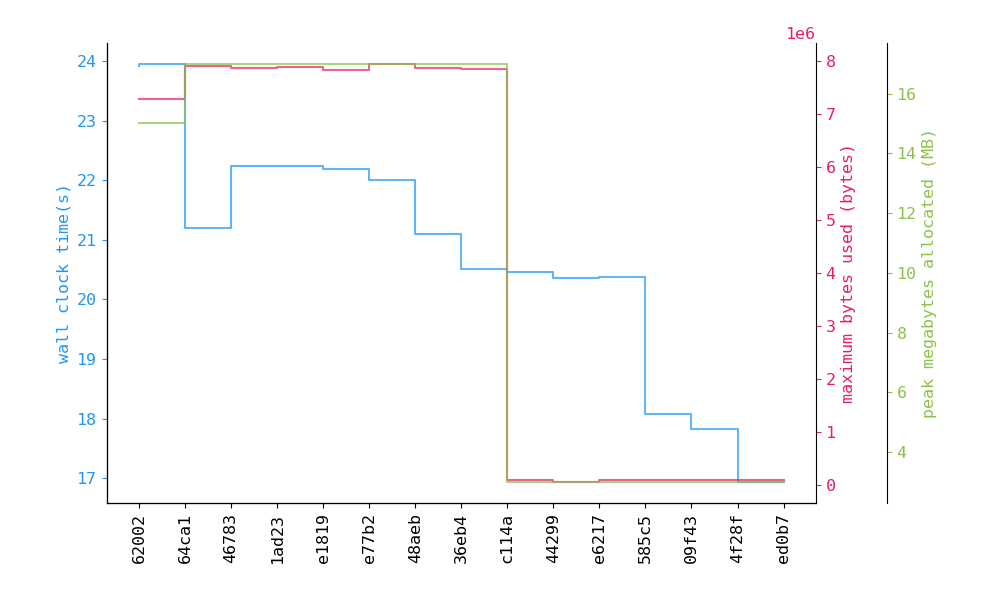
\includegraphics[height=0.6\textwidth]{./perfdata-gen.png}
\end{center}

%{\tiny
%\begin{minted}{text}
%64ca171 Replace CDouble with Double because its just a newtype.
%4678326 Restrict the export list to 'main'.
%1ad231a Mark entries of Ray and Sphere as UNPACK and Strict.
%e1819a6 Use a pattern synonym to unpack Refl in Sphere.
%e77b26f Change from maximum on a list to max.
%48aeb46 Convert erand48 to pure Haskell.
%36eb49e Change erand48 to IORefU.
%c114ace Rewrite the remaining IORef into a foldM.
%44299aa Remove the Data.Vector.Mutable by being purer.
%e62177b Set everything in smallpt to be strict.
%585c5cb Reduce to only effectful strictnesses.
%09f43c7 Remove Maybe from intersect(s)
%4f28fcc Hand unroll the fold in intersects.
%ed0b794 Marking interesects' f parameters strict.
%8309e4a Strategic application of strictness.
%7be5b4b Shorted erand48.
%578b83c Use LLVM backend.
%\end{minted}
%}
\end{frame}


\begin{frame}[fragile]{Takeaways}
\begin{itemize}
\item Haskell can be fast, given some sensitivity to performance.
\item Having performance leads to a faster baseline
      (unpacking, bang-patterns, \texttt{max},
      \texttt{LLVM} by default, exporting \texttt{main}, \dots)
\item Some others (unrolling \texttt{f}) is more subtle.
\item Accumulate optimizations to accrue performance wins.
%\item \href{https://docs.google.com/spreadsheets/d/1YhZlDRGvnCtN8UQf_0ItmgRWI9MhL21HDTlBEKqgWHc/edit#gid=0}{Raw Google Sheet of our transformations}
%\item \href{https://github.com/bollu/smallpths}{\texttt{github.com/bollu/smallpt-opt}}
\end{itemize}
\end{frame}
\end{document}
